%%% LaTeX Template: Article/Thesis/etc. with colored headings and special fonts
%%%
%%% Source: http://www.howtotex.com/
%%% Feel free to distribute this template, but please keep to referal to http://www.howtotex.com/ here.
%%% February 2011
%%%
%%% Modified Oct 2021 by CDM

%%%  Preamble
\documentclass[11pt,letterpaper]{article}
\usepackage[margin=1.0in]{geometry}
\usepackage[T1]{fontenc}
\usepackage[bitstream-charter]{mathdesign}
\usepackage[latin1]{inputenc}					
\usepackage{amsmath}						
\usepackage{xcolor}
\usepackage{cite}
\usepackage{hyphenat}
\usepackage{graphicx}
\usepackage{float}
\usepackage{subfigure}
\usepackage{sectsty}
\usepackage[compact]{titlesec} 
\usepackage[tablegrid]{vhistory}
\allsectionsfont{\color{accentcolor}\scshape\selectfont}

%%% Definitions
\definecolor{accentcolor}{rgb}{0.0,0.0,0.5} 
\newcommand{\teamname}{SegFault}
\newcommand{\productname}{Laser Harp}
\newcommand{\coursename}{CSE 4316: Senior Design I}
\newcommand{\semester}{Summer 2024}
\newcommand{\docname}{System Requirements Specification}
\newcommand{\department}{Department of Computer Science \& Engineering}
\newcommand{\university}{The University of Texas at Arlington}
\newcommand{\authors}{Simon Aguirre \\ Matthew Moran \\ Thomas Pinkney \\ Alex Tran}

%%% Headers and footers
\usepackage{fancyhdr}
	\pagestyle{fancy}						% Enabling the custom headers/footers
\usepackage{lastpage}	
	% Header (empty)
	\lhead{}
	\chead{}
	\rhead{}
	% Footer
	\lfoot{\footnotesize \teamname \ - \semester}
	\cfoot{}
	\rfoot{\footnotesize page \thepage\ of \pageref{LastPage}}	% "Page 1 of 2"
	\renewcommand{\headrulewidth}{0.0pt}
	\renewcommand{\footrulewidth}{0.4pt}

%%% Change the abstract environment
\usepackage[runin]{abstract}			% runin option for a run-in title
%\setlength\absleftindent{30pt}			% left margin
%\setlength\absrightindent{30pt}		% right margin
\abslabeldelim{\quad}	
\setlength{\abstitleskip}{-10pt}
\renewcommand{\abstractname}{}
\renewcommand{\abstracttextfont}{\color{accentcolor} \small \slshape}	% slanted text

%%% Start of the document
\begin{document}

%%% Cover sheet
{\centering \huge \color{accentcolor} \sc \textbf{\department \\ \university} \par}
\vspace{1 in}
{\centering \huge \color{accentcolor} \sc \textbf{\docname \\ \coursename \\ \semester} \par}
\vspace{0.5 in}
\begin{figure}[h!]
	\centering
   	
\includegraphics[width=0.50\textwidth]{images/Logo.png}
\end{figure}
\vspace{0.4 in}
{\centering \huge \color{accentcolor} \sc \textbf{\teamname \\ \productname} \par}
\vspace{0.25 in}
{\centering \large \sc \textbf{\authors} \par}
\newpage


%\vspace{1 in}
%\centerline{January 13th, 2012}
%\newpage

%%% Revision History
\begin{versionhistory}
  	\vhEntry{0.1}{10.01.2015}{GH}{document creation}
  	\vhEntry{0.2}{10.05.2015}{AT|GH}{complete draft}
  	\vhEntry{0.3}{10.12.2015}{AT|GH}{release candidate 1}
  	\vhEntry{1.0}{10.20.2015}{AT|GH|CB}{official release}
  	\vhEntry{1.1}{10.31.2015}{AL}{added customer change requests}
\end{versionhistory}
\newpage

%%% Table of contents
\setcounter{tocdepth}{3}
\tableofcontents
\newpage

%%% List of figures and tables (optional)
\listoffigures
%\listoftables
\newpage

\section{Product Concept}
\section{Product Concept}

This section describes the purpose, use, and intended user audience for the laser harp. The laser harp is a musical instrument designed to provide an innovative and engaging way to create music using laser technology. Users of the laser harp will be able to produce sounds by interrupting laser beams, simulating the plucking of strings on a traditional harp. This section provides a high-level statement of the product concept, outlining what it is intended to do and how it is intended to be used.

\subsection{Purpose and Use}
The laser harp is designed to provide an interactive musical experience by using laser beams as virtual strings. When a laser beam is interrupted, the system detects the interruption and plays a corresponding musical note. The purpose of the laser harp is to offer a unique and modern approach to playing music, combining elements of traditional string instruments with advanced technology. It is expected to be used in educational settings to inspire interest in STEM subjects, as well as by musicians and hobbyists looking for an innovative way to create music.

\subsection{Intended Audience}
The intended audience for the laser harp includes educational institutions, music enthusiasts, and hobbyists. In educational settings, the laser harp can be used as a tool to engage students in learning about music, electronics, and programming. Music enthusiasts and hobbyists will appreciate the creative possibilities offered by the laser harp, as it provides a new way to experiment with musical composition and performance. The product is designed for general use and can be integrated into various educational and recreational activities.

\begin{figure}[h!]
	\centering
   	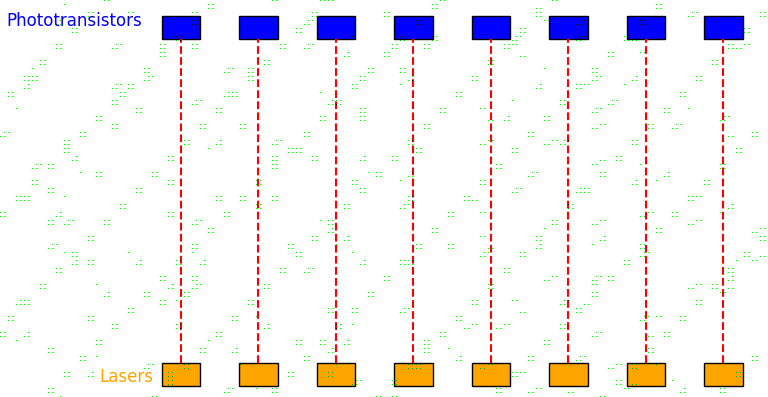
\includegraphics[width=0.60\textwidth]{images/Design}
    \caption{Laser Harp conceptual drawing}
\end{figure}

\newpage
\section{Product Description}
This section provides a description of your product and defines it's primary features and functions. The purpose is to give the document reader/reviewer enough information about the product to allow them to easily follow the specification of requirements found in the remainder of the document. Your header for this section should introduce the section with a brief statement such as: "This section provides the reader with an overview of X. The primary operational aspects of the product, from the perspective of end users, maintainers and administrators, are defined here. The key features and functions found in the product, as well as critical user interactions and user interfaces are described in detail." Using words, and pictures or graphics where possible, specify the following:

\subsection{Features \& Functions}
What the product does and does not do. Specify in words what it looks like, referring to a conceptual diagram/graphic (Figure X).  Define the principle parts/components of the product. Specify the elements in the diagram/graphic that are part(s) of this product as well as any associated external elements (e.g., the Internet, an external web server, a GPS satellite, etc.)

\subsection{External Inputs \& Outputs}
Describe critical external data flows. What does your product require/expect to receive from end users or external systems (inputs), and what is expected to be created by your product for consumption by end users or external systems (outputs)? In other words, specify here all data/information to flow into and out of your systems. A table works best here, with rows for each critical data element, and columns for name, description and use.

\subsection{Product Interfaces}
Specify what all operational (visible) interfaces look like to your end-user, administrator, maintainer, etc. Show sample/mocked-up screen shots, graphics of buttons, panels, etc. Refer to the critical external inputs and outputs described in the paragraph above.

\newpage
\section{Customer Requirements}
This project aims to design and develop an innovative laser harp that serves as both an educational tool and a musical instrument. Customer requirements for this project are established to ensure the product meets the needs of its intended users, which include educational institutions, music enthusiasts, and hobbyists. These requirements outline the essential features and functionalities that the product must deliver to achieve user satisfaction and fulfill its purpose. Any changes to these requirements must be agreed upon by the project stakeholders, including the customer, sponsors, and the development team.

\subsection{Laser String Detection}
\subsubsection{Description}
The laser harp must accurately detect when a laser string is interrupted (plucked) and identify which specific string was interrupted. This detection must be reliable under various lighting conditions to ensure consistent performance during use.
\subsubsection{Source}
Customer, CSE Senior Design project specifications
\subsubsection{Constraints}
- **Economic:**: The solution should be cost-effective, using commercially available components.
Environmental: Must operate reliably in indoor environments with variable lighting.
Health & Safety: The lasers used must be safe for use around humans, adhering to Class 1 laser safety standards.
Manufacturability: The system should be easy to assemble and maintain.
\subsubsection{Standards}
IEC 60825-1:2014 Safety of Laser Products
IEEE 802.3 for electronic components
\subsubsection{Priority}
Critical


\subsection{Audio Output}
\subsubsection{Description}
The laser harp must produce a sound corresponding to the interrupted laser string. The sounds should be pre-recorded harp notes stored in .wav format and played through an audio output system. The system should support simultaneous playback of multiple notes to create chords.
\subsubsection{Source}
Customer, CSE Senior Design project specifications
\subsubsection{Constraints}
- **Economic:**: Use of open-source libraries and cost-effective audio hardware.
Environmental: Must function reliably in standard indoor environments.
Health & Safety: Audio output should be within safe hearing levels
\subsubsection{Standards}
WAV File Format Specification
OpenAL Standard for Audio Playback
\subsubsection{Priority}
Critical


\subsection{Portable}
\subsubsection{Description}
The laser harp must be portable, allowing it to be easily transported and set up in different locations. The device should be lightweight and compact without compromising functionality.
\subsubsection{Source}
specified team member (Simon Aguirre)
\subsubsection{Constraints}
- **Economic:**: Materials used should balance cost and durability.
Environmental: Device should withstand minor impacts and vibrations during transport.
Health & Safety: Ensure safe handling and transport.
\subsubsection{Standards}
IEC 60068-2-31: Test for shock and bump for equipment
\subsubsection{Priority}
High


\subsection{Power Supply}
\subsubsection{Description}
The laser harp must operate on a rechargeable battery with a minimum of 4 hours of continuous use per charge. It should also support operation while charging.
\subsubsection{Source}
specified team member (Matthew Moran)
\subsubsection{Constraints}
- **Economic:**: Use cost-effective and safe rechargeable battery solutions.
Environmental: Battery should be compliant with environmental regulations for disposal.
Health & Safety: Battery must meet safety standards to prevent overheating and other hazards.
\subsubsection{Standards}
IEC 62133-2:2017 for rechargeable battery safety
\subsubsection{Priority}
Moderate


\subsection{User Interface}
\subsubsection{Description}
The laser harp must include a user interface (UI) that allows users to calibrate the laser strings, adjust volume, and select different sound profiles. The UI should be intuitive and accessible.
\subsubsection{Source}
specified team member (Matthew Moran)
\subsubsection{Constraints}
- **Economic:**: Development should utilize open-source UI frameworks.
Environmental: Must be usable in typical classroom and home settings.
Social: The UI design should be inclusive and accessible to users with different needs.
\subsubsection{Standards}
Web Content Accessibility Guidelines (WCAG) 2.1 for UI accessibility
\subsubsection{Priority}
Low


\subsection{Wireless Connectivity}
\subsubsection{Description}
Future versions of the laser harp should include wireless connectivity options such as Bluetooth or Wi-Fi for remote control and updates.
\subsubsection{Source}
None
\subsubsection{Constraints}
- **Economic:**: Ensure cost-effective implementation of wireless modules.
Environmental: Reliable operation in typical indoor environments.
Health & Safety: Adhere to wireless communication safety standards.
\subsubsection{Standards}
IEEE 802.11 for Wi-Fi
Bluetooth SIG standards for Bluetooth
\subsubsection{Priority}
Future

\newpage
\section{Packaging Requirements}
The packaging requirements for the laser harp project identify how the delivered product will be packaged for delivery to the end-user and how it will "look" when finished and delivered. For example, the software required for operation will be pre-loaded on the included microSD card. The product will be delivered in a single package, ensuring all components are included and protected during shipping. Some components may require user assembly, with detailed instructions provided. The device will feature company branding and a professional finish. Care is taken not to duplicate requirements found in other sections of this document.


\subsection{Pre-loaded Software}
\subsubsection{Description}
The software required for the operation of the laser harp must be pre-loaded onto the included microSD card. This includes the operating system, necessary drivers, and the laser harp control software.
\subsubsection{Source}
Development Team, Customer
\subsubsection{Constraints}
Economic: Pre-loading software reduces the need for end-user installation support, lowering post-sale support costs.\\
Technical: The software must be thoroughly tested to ensure it works out-of-the-box.\\
Usability: Ensures a seamless user experience by reducing setup complexity.
\subsubsection{Standards}
ISO/IEC 25010: Systems and software Quality Requirements and Evaluation (SQuaRE) - System and software quality models.
\subsubsection{Priority}
High


\subsection{Single Package Delivery}
\subsubsection{Description}
All hardware components of the laser harp must be delivered in a single package. This package should include the main unit, power supply, USB receiver, user manual, and any necessary cables.
\subsubsection{Source}
Customer, Sponsor
\subsubsection{Constraints}
Economic: Consolidating packaging reduces shipping costs and potential damage during transport.\\
Environmental: Packaging materials should be recyclable to minimize environmental impact.\\
Health & Safety: Packaging must protect the components from damage during shipping and handling.
\subsubsection{Standards}
ISO 11607-1: Packaging for terminally sterilized medical devices - Requirements for materials, sterile barrier systems, and packaging systems.
\subsubsection{Priority}
High


\subsection{Customer Support Information}
\subsubsection{Description}
The package must include customer support information, such as a toll-free support number, email address, and website URL for troubleshooting and assistance.
\subsubsection{Source}
Customer, Sponsor
\subsubsection{Constraints}
Economic: Including support information helps reduce the need for returns and enhances customer satisfaction.\\
Usability: Information must be easy to find and clearly printed in the user manual.
\subsubsection{Standards}
ISO 10002 Quality management - Customer satisfaction - Guidelines for complaints handling in organizations.
\subsubsection{Priority}
Moderate/Future


\subsection{User-assembled Components}
\subsubsection{Description}
Some components of the laser harp, such as the frame and the laser modules, will be user-assembled. Detailed assembly instructions must be provided to guide users through this process.
\subsubsection{Source}
Development Team
\subsubsection{Constraints}
Economic: User assembly reduces manufacturing and shipping costs.\\
Usability: Instructions must be clear and easy to follow, with diagrams and step-by-step guidance.\\
Health & Safety: Assembly instructions must include safety warnings and precautions.
\subsubsection{Standards}
ISO 7000 Graphical symbols for use on equipment - Registered symbols.
\subsubsection{Priority}
Moderate


\subsection{Branding and Appearance}
\subsubsection{Description}
The laser harp must feature the company logo and branding. The main unit should be painted in the company’s colors and have a professional finish.
\subsubsection{Source}
Sponsor
\subsubsection{Constraints}
Economic: Branding should not significantly increase manufacturing costs.\\
Usability: The branding should not obscure any functional parts of the device.\\
Aesthetics: The device should have a professional and attractive appearance to enhance customer satisfaction.
\subsubsection{Standards}
ISO 3864-1: Graphical symbols - Safety colors and safety signs.
\subsubsection{Priority}
Low

\newpage
\section{Performance Requirements}
Include a header paragraph specific to your product here. Performance requirements address items such as: how fast specific critical operations must complete; how long it takes to start/stop activities; how long the battery must last; maximum time it must take to set up; etc.

\subsection{Requirement Name}
\subsubsection{Description}
Detailed requirement description...
\subsubsection{Source}
Source
\subsubsection{Constraints}
Detailed description of applicable constraints...
\subsubsection{Standards}
List of applicable standards
\subsubsection{Priority}
Priority
\newpage
\section{Safety Requirements}
The safety requirements for the laser harp project ensure that the product is safe for use and minimizes any potential hazards. These requirements address various safety aspects such as avoiding exposure to harmful components, ensuring safe handling of electrical connections, and implementing procedures to prevent accidents during the development and use of the product.

\subsection{Laboratory Equipment Lockout/Tagout (LOTO) Procedures}
\subsubsection{Description}
Any fabrication equipment used in the development of the project shall be operated in accordance with OSHA standard LOTO procedures. Locks and tags are installed on all equipment items that present use hazards, and only the course instructor or designated teaching assistants may remove a lock. All locks will be immediately replaced once the equipment is no longer in use.
\subsubsection{Source}
CSE Senior Design laboratory policy
\subsubsection{Constraints}
Equipment usage, due to lock removal policies, will be limited to the availability of the course instructor and designated teaching assistants.
\subsubsection{Standards}
Occupational Safety and Health Standards 1910.147 - The control of hazardous energy (lockout/tagout).
\subsubsection{Priority}
Critical

\subsection{National Electric Code (NEC) Wiring Compliance}
\subsubsection{Description}
Any electrical wiring must comply with all requirements specified in the National Electric Code. This includes wire runs, insulation, grounding, enclosures, over-current protection, and all other specifications.
\subsubsection{Source}
CSE Senior Design laboratory policy
\subsubsection{Constraints}
High voltage power sources, as defined in NFPA 70, will be avoided as much as possible to minimize potential hazards.
\subsubsection{Standards}
NFPA 70
\subsubsection{Priority}
Critical

\subsection{No Direct Eye Exposure to Lasers}
\subsubsection{Description}
The laser harp must be designed to prevent any direct eye exposure to laser beams. Class 1 lasers, which are safe under all conditions of normal use, will be used to ensure user safety.
\subsubsection{Source}
Development Team
\subsubsection{Constraints}
Ensure all laser components are securely mounted and aligned to prevent accidental exposure. Safety warnings and guidelines must be included in the user manual.
\subsubsection{Standards}
IEC 60825-1:2014 Safety of Laser Products
\subsubsection{Priority}
Critical

\subsection{Grounding of Electrical Connections}
\subsubsection{Description}
All electrical connections within the laser harp must be properly grounded to avoid any risk of electrical shock. This includes ensuring all exposed metal parts are connected to a common ground point.
\subsubsection{Source}
Development Team
\subsubsection{Constraints}
All electrical components must be installed in accordance with grounding best practices. Regular inspections should be performed to ensure grounding integrity.
\subsubsection{Standards}
IEC 60364-5-54:2011 Low-voltage electrical installations - Part 5-54: Selection and erection of electrical equipment - Earthing arrangements and protective conductors
\subsubsection{Priority}
High

\subsection{Use of Non-Toxic Materials}
\subsubsection{Description}
All materials used in the construction of the laser harp must be non-toxic and safe for handling. This includes avoiding the use of hazardous chemicals and ensuring that all parts are free from sharp edges.
\subsubsection{Source}
Development Team, Customer
\subsubsection{Constraints}
Materials must comply with safety regulations and standards for non-toxicity. The use of environmentally friendly materials is encouraged.
\subsubsection{Standards}
REACH Regulation (EC) No 1907/2006 concerning the Registration, Evaluation, Authorisation and Restriction of Chemicals
\subsubsection{Priority}
High

\subsection{Packaging of Electrical Components}
\subsubsection{Description}
All electrical components must be securely packaged to prevent damage during shipping and handling. This includes using appropriate insulation and ensuring that components are protected from moisture and impact.
\subsubsection{Source}
Development Team
\subsubsection{Constraints}
Packaging materials must be chosen to provide adequate protection while being cost-effective. The use of recyclable packaging is preferred.
\subsubsection{Standards}
IEC 60215:2016 Safety requirements for radio transmitting equipment
\subsubsection{Priority}
Moderate

\newpage
\section{Security Requirements}
The security requirements for the laser harp project ensure that all aspects of information security and privacy are addressed. This includes the implementation of encryption standards, secure data storage procedures, robust authentication mechanisms, and strong password policies to protect user data and system integrity.

\subsection{Data Encryption}
\subsubsection{Description}
All sensitive data transmitted and stored by the laser harp system must be encrypted using industry-standard encryption algorithms. This includes user settings, calibration data, and any other personal information.
\subsubsection{Source}
Development Team
\subsubsection{Constraints}
Encryption algorithms must be efficient to not degrade system performance. Encryption keys must be securely managed and stored.
\subsubsection{Standards}
AES (Advanced Encryption Standard) - NIST FIPS 197
\subsubsection{Priority}
Critical


\subsection{Secure Data Storage}
\subsubsection{Description}
All data stored on the laser harp system must be secured to prevent unauthorized access. This includes the use of secure storage mechanisms and regular data backups.
\subsubsection{Source}
Development Team
\subsubsection{Constraints}
Secure storage solutions must be cost-effective and reliable. Data backups must be performed regularly and stored securely.
\subsubsection{Standards}
ISO/IEC 27001:2013 - Information security management systems
\subsubsection{Priority}
High


\subsection{Secure Firmware Updates}
\subsubsection{Description}
Firmware updates for the laser harp system must be delivered securely to prevent unauthorized modifications. This includes the use of digital signatures to verify the integrity and authenticity of the firmware.
\subsubsection{Source}
Development Team
\subsubsection{Constraints}
Firmware update mechanisms must be reliable and user-friendly to ensure users can easily apply updates.
\subsubsection{Standards}
NIST SP 800-147 - BIOS Protection Guidelines
\subsubsection{Priority}
Moderate

\newpage
\section{Maintenance \& Support Requirements}
The maintenance and support requirements for the laser harp project are designed to ensure that the product remains functional, reliable, and user-friendly after delivery. These requirements outline the necessary steps and resources for maintaining the product, correcting errors, and providing support to end users. The goal is to provide a clear plan for ongoing product care, including troubleshooting, repair, and updates. This involves defining who will be responsible for maintenance, the necessary tools and documentation, and the standards to be followed.


\subsection{Source Code}
\subsubsection{Description}
The source code for the laser harp's software must be made available to the maintenance team. This includes all code related to the operation of the laser detection, audio playback, and user interface components.
\subsubsection{Source}
Development Team
\subsubsection{Constraints}
- **Economic:**: Secure storage and version control systems must be maintained to manage the source code.
Security: Access to the source code should be restricted to authorized personnel to prevent unauthorized changes or misuse.
Documentation: The source code must be well-documented to ensure maintainers can understand and modify it as needed.
\subsubsection{Standards}
IEEE 828: Configuration Management for Systems and Software Engineering.
\subsubsection{Priority}
Critical


\subsection{Maintenance Tools}
\subsubsection{Description}
Specific tools and equipment must be available for maintaining the laser harp. This includes standard electronic repair tools (soldering iron, multimeter, oscilloscope) as well as any specialized tools required for working with the laser and audio components.
\subsubsection{Source}
Development Team
\subsubsection{Constraints}
- **Economic:**: Budget for the procurement and maintenance of necessary tools.
Health & Safety: Ensure all maintenance tools meet safety standards to prevent accidents during use.
- **Usability:**: Tools should be user-friendly and suitable for the technical skills of the maintenance personnel.
\subsubsection{Standards}
OSHA Standards: Occupational Safety and Health Administration standards for tool safety.
\subsubsection{Priority}
High


\subsection{Software and Environment Requirements}
\subsubsection{Description}
The maintenance of the laser harp's software requires specific development environments and libraries. This includes the programming languages used (e.g., C++, Python), development tools (e.g., Visual Studio Code), and audio libraries (e.g., SFML).
\subsubsection{Source}
Development Team
\subsubsection{Constraints}
- **Economic:**: Ensure that all necessary software licenses are obtained and maintained.
- **Technical:**: The development environment must be compatible with the software components of the laser harp.
- **Usability:**: The environment should be configured to facilitate easy development, testing, and deployment of updates.
\subsubsection{Standards}
IEEE 14764: Software Engineering - Software Life Cycle Processes - Maintenance.
\subsubsection{Priority}
High


\subsection{Maintenance Documentation}
\subsubsection{Description}
Comprehensive maintenance documentation must be provided to guide users and support personnel in troubleshooting and repairing the laser harp. This documentation should include user manuals, troubleshooting guides, repair procedures, and detailed diagrams of the system.
\subsubsection{Source}
Development Team
\subsubsection{Constraints}
- **Economic:**: The creation and upkeep of detailed documentation must be budgeted for, including potential updates as the product evolves.
- **Technical:**: Documentation must be thorough and accessible, using clear language and visuals to aid understanding.
- **Usability:**: Documentation should be designed to be user-friendly, ensuring that users of varying technical skill levels can effectively use and maintain the product.
\subsubsection{Standards}
ISO/IEC 26514: Systems and software engineering — Requirements for designers and developers of user documentation.
\subsubsection{Priority}
Moderate


\subsection{Technical Support}
\subsubsection{Description}
A dedicated support team must be available to provide technical assistance to users. This team should be trained in the operation and maintenance of the laser harp and capable of addressing common issues.
\subsubsection{Source}
Customer, Development Team
\subsubsection{Constraints}
- **Economic:**: Budget for hiring and training support personnel.
- **Technical:**: Support personnel must have a deep understanding of the laser harp's components and software.
- **Usability:**: Support services should be easily accessible to users, with multiple contact methods available (e.g., phone, email, online chat).
\subsubsection{Standards}
ISO 20000: Information technology — Service management.
\subsubsection{Priority}
Low/Future

\newpage
\section{Other Requirements}
This section includes any additional requirements necessary for the laser harp to be deemed complete. These requirements cover aspects such as customer setup and configuration, product architecture and design, modularity, extensibility, and portability. Ensuring these elements are addressed is crucial for the overall functionality and future-proofing of the product.


\subsection{Quality Assurance}
\subsubsection{Description}
The laser harp must undergo rigorous testing and quality assurance processes to ensure reliability and performance. This includes functional testing, stress testing, and user acceptance testing.
\subsubsection{Source}
Development Team
\subsubsection{Constraints}
Economic: Allocate sufficient budget for comprehensive testing procedures.
Technical: Utilize appropriate testing frameworks and tools.
Usability: Testing processes should simulate real-world usage scenarios.
\subsubsection{Standards}
ISO/IEC/IEEE 29119: Software Testing standards.
\subsubsection{Priority}
High


\subsection{Setup}
\subsubsection{Description}
The laser harp must include a straightforward setup and configuration process for end users. This process should be well-documented and easy to follow, allowing users to quickly assemble and configure the harp for use.
\subsubsection{Source}
Customer, Development Team
\subsubsection{Constraints}
Economic: The setup process should not require expensive tools or components.
Usability: Instructions must be clear and accessible to users of varying technical skill levels.
Time: Setup should be quick, ideally taking no more than 30 minutes.
\subsubsection{Standards}
ISO 9241-11: Ergonomics of human-system interaction – Part 11: Usability: Definitions and concepts.
\subsubsection{Priority}
High


\subsection{Extensible}
\subsubsection{Description}
The software and hardware architecture of the laser harp must be extensible to allow for future enhancements and additional features. This includes the ability to add new sound profiles, connectivity options, and user interface improvements
\subsubsection{Source}
Development Team
\subsubsection{Constraints}
Economic: Extensibility should not significantly increase initial development costs.
Technical: The system architecture must be designed to support easy integration of new features.
Usability: New features should be easily accessible to end users.
\subsubsection{Standards}
IEEE 14764: Software Engineering – Software Life Cycle Processes – Maintenance.
\subsubsection{Priority}
Moderate


\subsection{Modular}
\subsubsection{Description}
The design of the laser harp must be modular, allowing for easy replacement or upgrading of components. This includes both hardware components (e.g., lasers, sensors) and software modules.
\subsubsection{Source}
Development Team
\subsubsection{Constraints}
Economic: Modular design should not significantly increase the cost of the product.
Technical: Modules must be easily interchangeable and compatible with the overall system.
Usability: Users should be able to replace or upgrade modules without specialized technical knowledge.
\subsubsection{Standards}
IEC 61131-3: Programmable controllers – Part 3: Programming languages.
\subsubsection{Priority}
Moderate


\subsection{Portable}
\subsubsection{Description}
The software for the laser harp must be portable across various platforms, including Windows, Linux, macOS, and Unix. This ensures that the product can be used in diverse environments and is accessible to a wide range of users.
\subsubsection{Source}
Customer, Development Team
\subsubsection{Constraints}
Economic: Development and testing across multiple platforms should be budgeted for.
Technical: The software must be compatible with different operating systems and their respective libraries.
Usability: The user experience should be consistent across all supported platforms.
\subsubsection{Standards}
IEEE 1003.1: POSIX standard for portability.
\subsubsection{Priority}
Low/Future

\newpage
\section{Future Items}
\subsection{Wireless Connectivity}
\subsubsection{Description}
Future versions of the laser harp should include wireless connectivity options such as Bluetooth or Wi-Fi for remote control and updates.
\subsubsection{Source}
None
\subsubsection{Constraints}
- **Economic:**: Ensure cost-effective implementation of wireless modules.
Environmental: Reliable operation in typical indoor environments.
Health & Safety: Adhere to wireless communication safety standards.
\subsubsection{Standards}
IEEE 802.11 for Wi-Fi
Bluetooth SIG standards for Bluetooth
\subsubsection{Priority}
Future


\subsection{Customer Support Information}
\subsubsection{Description}
The package must include customer support information, such as a toll-free support number, email address, and website URL for troubleshooting and assistance.
\subsubsection{Source}
Customer, Sponsor
\subsubsection{Constraints}
- **Economic:** Including support information helps reduce the need for returns and enhances customer satisfaction.
- **Usability:** Information must be easy to find and clearly printed in the user manual.
\subsubsection{Standards}
- **ISO 10002:** Quality management - Customer satisfaction - Guidelines for complaints handling in organizations.
\subsubsection{Priority}
Moderate/Future


\subsection{Technical Support}
\subsubsection{Description}
A dedicated support team must be available to provide technical assistance to users. This team should be trained in the operation and maintenance of the laser harp and capable of addressing common issues.
\subsubsection{Source}
Customer, Development Team
\subsubsection{Constraints}- **Economic:**: Budget for hiring and training support personnel.
- **Technical:**: Support personnel must have a deep understanding of the laser harp's components and software.
- **Usability:**: Support services should be easily accessible to users, with multiple contact methods available (e.g., phone, email, online chat).
\subsubsection{Standards}
ISO 20000: Information technology — Service management.
\subsubsection{Priority}
Low/Future


\subsection{Portable}
\subsubsection{Description}
The software for the laser harp must be portable across various platforms, including Windows, Linux, macOS, and Unix. This ensures that the product can be used in diverse environments and is accessible to a wide range of users.
\subsubsection{Source}
Customer, Development Team
\subsubsection{Constraints}
- **Economic:**: Development and testing across multiple platforms should be budgeted for.
- **Technical:**: The software must be compatible with different operating systems and their respective libraries.
- **Usability:**: The user experience should be consistent across all supported platforms.
\subsubsection{Standards}
IEEE 1003.1: POSIX standard for portability.
\subsubsection{Priority}
Low/Future

\newpage

\end{document}
